\documentclass[../../main.tex]{subfiles}
\begin{document}

\subsection*{7.7}
Due griglie $G_1$ e $G_2$ metalliche parallele molto estese distanti $d = 4\ cm$, tra le quali è applicata una ddp V separando due regioni in cui esiste un campo magnetico $B=0.8\ T$ uniforme, ortogonale al foglio.\\In un punto $A_1$ viene iniettato un protone con $vel = v_1$ che a $t_0 = 0$ attraversa la griglia perpendicolarmente.
\\Dopo un tempo $t = 1.22 *10^{-7}\ s$ il protone riattraversa $G_1$ nello stesso verso in un punto $A_2$ distante $h=5.2\ cm$ da $A_1$.
\\Descrivere la traiettoria percorsa dal protone $A_1$ e $A_2$ e calcolare la d.d.p. V applicata tra le griglie e la velocità $v_1$ e $v_2$ elle 2 regioni in cui c'è campo.
\\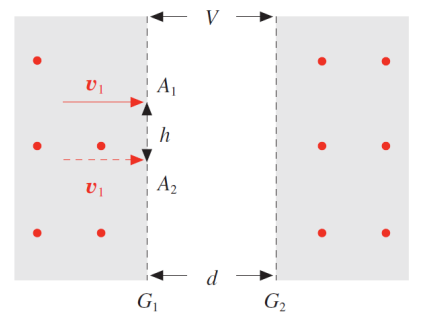
\includegraphics[scale=0.3]{e_7_7_0.png}
\\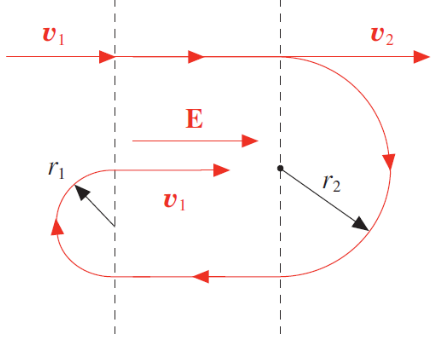
\includegraphics[scale=0.3]{e_7_7_1.png}
\subsubsection*{Formule utilizzate}
\subsubsection*{Soluzione punto a}
$\Delta = \frac{1}{2}mv_2^2 - \frac{1}{2}mv_1^2$
\\$d=v_mt$
\\$v_m=\frac{v_2+v_1}{m}$
\\$h = \vec{A_1A_2} = 2(r_2-r_1)$
\\$\Delta E_k = \frac{1}{2}mv_2^2-\frac{1}{2}mv_1^2=q\Delta v$
\\$\Delta V= \frac{\frac{1}{2}m(v_2^2-v_1^2)}{q}$
\subsubsection*{Soluzione punto b}
\newpage

\end{document}